% Section content template for individual Educative lessons
% This file contains the actual content for a specific section
% Generated from Educative API section content

% Section: Class Diagram for the Car Rental System
% Section ID: 5607380186562560
% Section Slug: class-diagram-for-the-car-rental-system
% Generated: 2025-12-12T14:51:39.206333

Based on the given requirements, we'll create the class diagram for the car rental system. In the class diagram, we will first identify the system's classes (concrete, abstract, or associated) and interfaces. Then , we will determine the relationship between them according to the requirements in the previous lesson.

\subsection{Components of a car rental system}\label{t2RTZJSykCu3qCiyNEfXV}
\\
As mentioned, we'll design the car rental system using a bottom-up approach.

\subsubsection{Address and person}\label{UPV_LcgZzhhT_6y1HBAbq}
\\
The \texttt{Address} class is a reusable value object representing a physical address within the car rental system. This class standardizes storing and referencing addresses for customers, staff, and branches. It contains attributes such as street address, city, state/province, postal/zip code, and country.
\\
The \texttt{Person} class is an abstract base class that encapsulates common personal information for all individuals in the system, including customers, receptionists, and workers. This class centralizes attributes and methods shared by everyone in the system, promoting code reuse and maintainability. The class representation of \texttt{Address} and \texttt{Person} is given below:
\\
No change in the class representation of these classes.

\begin{figure}[htbp]
 \centering
 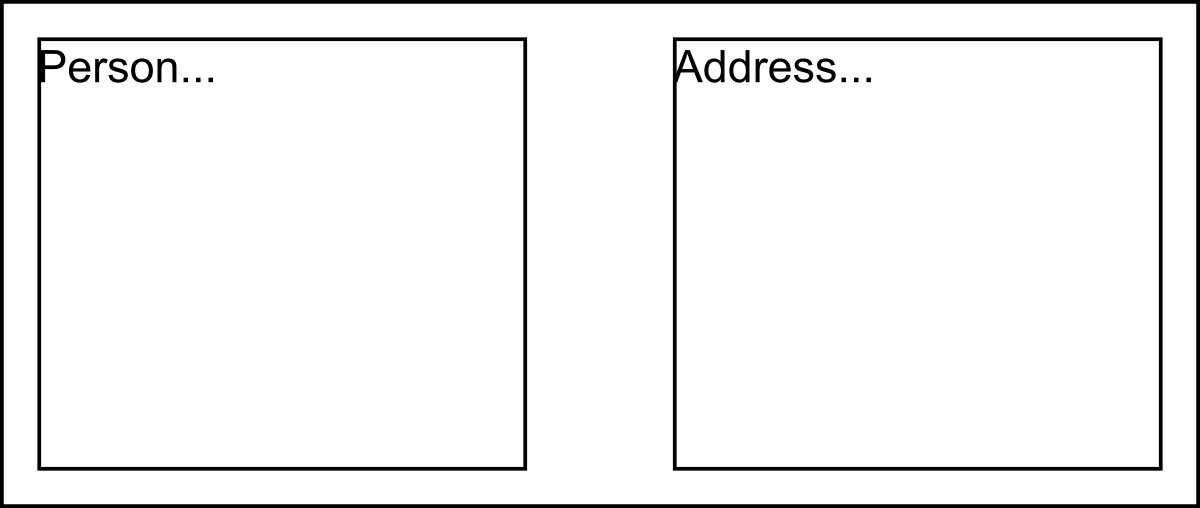
\includegraphics[width=0.5\textwidth]{Images/chapter_15/section_5607380186562560/5552865658798080.png}
 \caption{The class diagram of the Address and Person classes}
\end{figure}

\textbf{R1:} The system supports two main user roles: customers and receptionists.
\\
\textbf{R4:} The system must record every reservation, including the customer details and the date/time a vehicle is issued.
\\
\textbf{R12:} The system must support the management of multiple branches in different cities and locations

\subsubsection{Account}\label{unp3y-QDa6psC3OH52thY-1}
\\
The \texttt{Account} class represents a person's login and system access credentials. It is an abstract class because only specific user roles (customer, receptionist, worker) log into the system. The
\texttt{Account} class manages authentication, authorization, and account state. This class has members like account ID, password, account status, etc.
\\
The \texttt{Customer} class represents customers who can register, log in, make vehicle reservations, manage their bookings, make payments, and receive notifications. The
\texttt{Receptionist} is responsible for managing vehicles, reservations, and branch operations. Receptionists inherit all \texttt{Customer} privileges and can administer inventory and operations for their branch.
\\
The class representation of \texttt{Account} and its subclasses is given below:

\begin{figure}[htbp]
 \centering
 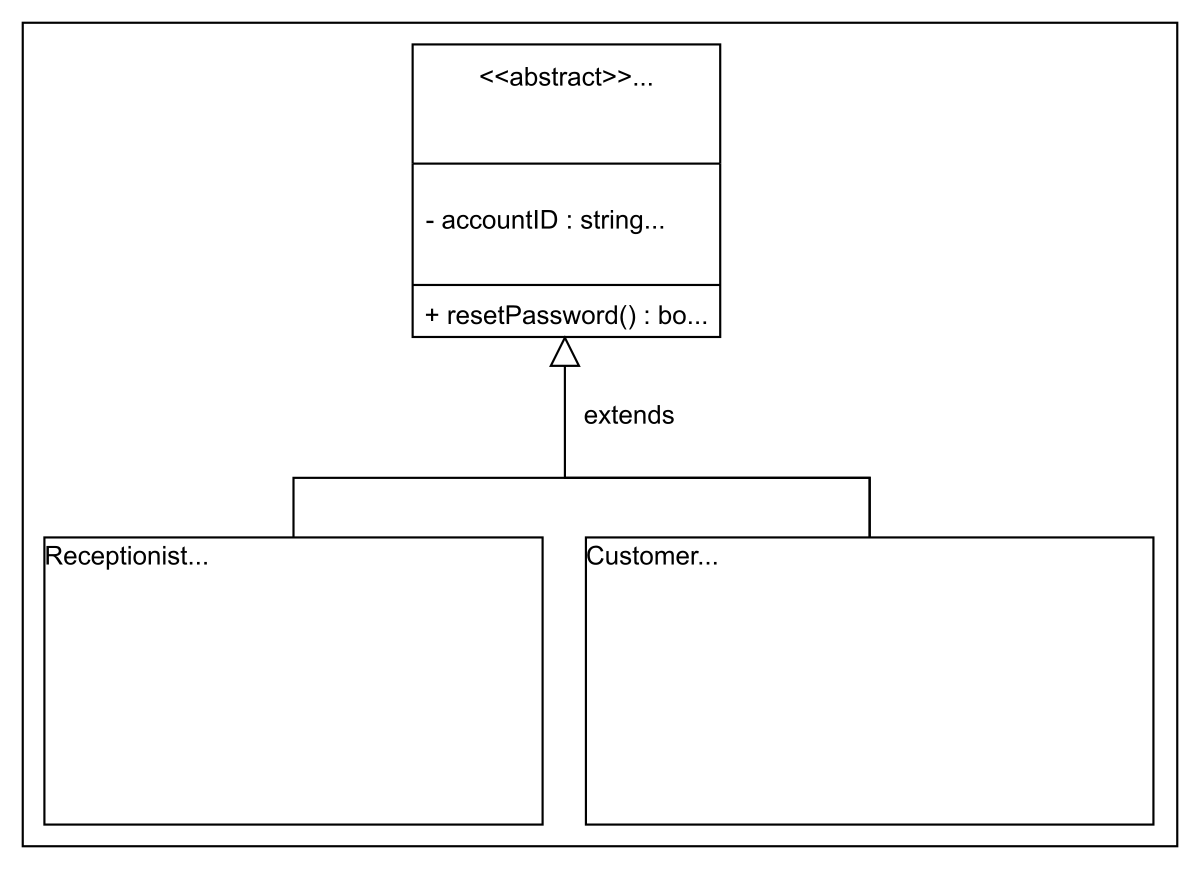
\includegraphics[width=0.5\textwidth]{Images/chapter_15/section_5607380186562560/6120918395781120.png}
 \caption{The class diagram of the Account class}
\end{figure}

\textbf{R1:} The system supports two main user roles: customers and receptionists.
\\
\textbf{R4:} The system must record every reservation, including the customer details and the date/time a vehicle is issued.
\\
\textbf{R6:} Customers can cancel their reservations at any time before the pickup date, subject to company policies.

\subsubsection{Driver}\label{P4z8rT5n_HGoR9L5X9bLr-1}
\\
We will have a \texttt{Driver} class as we are designing the car rental problem. A customer can request an additional driver at the time of reservation. The class diagram is shown below:

\begin{figure}[htbp]
 \centering
 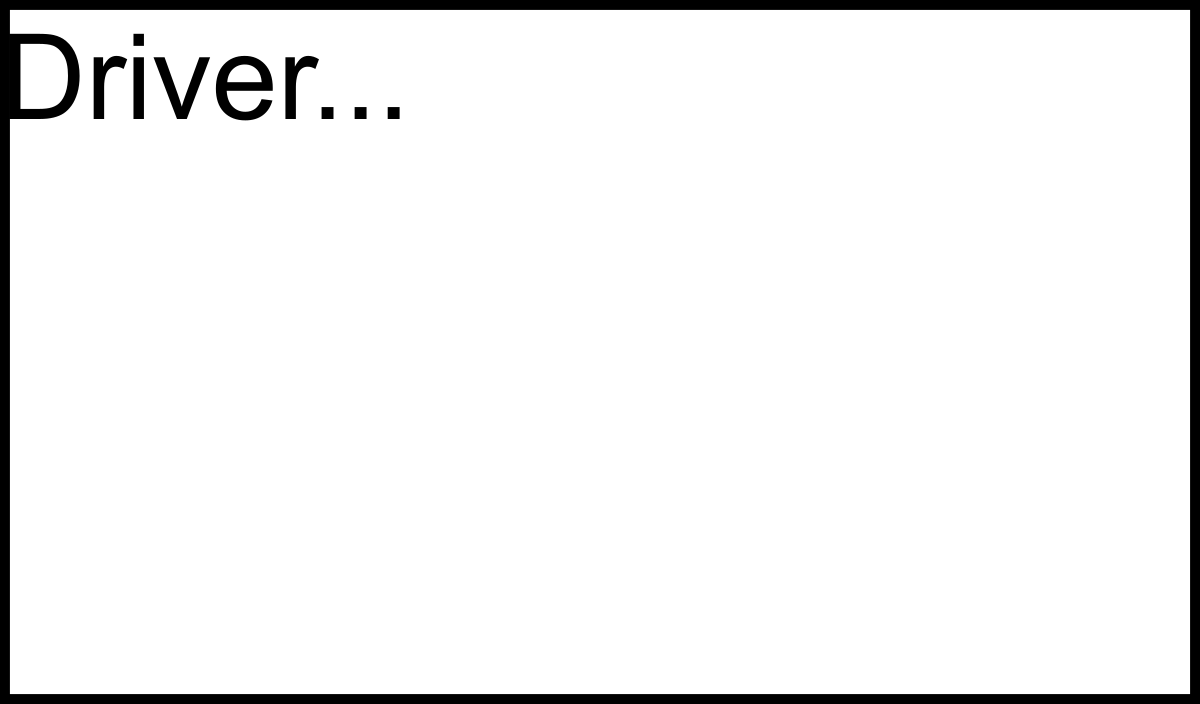
\includegraphics[width=0.5\textwidth]{Images/chapter_15/section_5607380186562560/6339149135347712.png}
 \caption{The class diagram of the Driver class}
\end{figure}

\subsubsection{Vehicle}\label{RmMg5DmgsexUkULnUt5st}
\\
Our car rental system should have a vehicle object according to the requirements. The vehicle can be of four types: a car, a truck, a van, or a motorcycle. For this purpose, we'll create \texttt{Vehicle} as an abstract class and \texttt{Car}, \texttt{Truck}, \texttt{Van}, and \texttt{Motorcycle} as its subclasses, as shown in the figure below:

\begin{figure}[htbp]
 \centering
 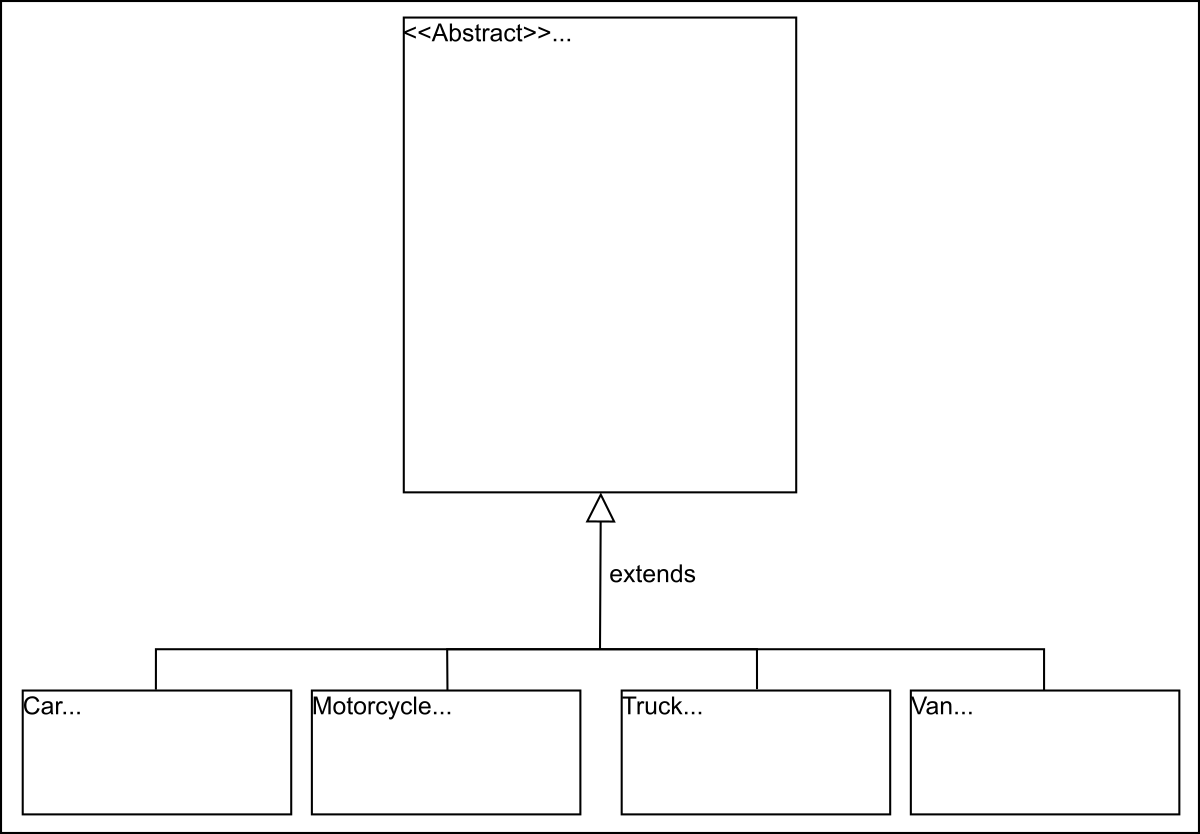
\includegraphics[width=0.5\textwidth]{Images/chapter_15/section_5607380186562560/6116384205701120.png}
 \caption{The class diagram of Vehicle and its derived classes}
\end{figure}

\textbf{R2:} The system should handle multiple types of vehicles. Initially, it should cater to cars, trucks, vans, and motorcycles.

\subsubsection{Equipment}\label{RaL7OUsivwIviWcLABJne-1}
\\
\texttt{Equipment} is an abstract class that stores information about different types of equipment that can be added to the reservation. For simplicity, we'll assume three types of equipment, i.e., navigation, child seat, and ski rack. The class diagram for \texttt{Equipment} and its subclasses is as follows:

\begin{figure}[htbp]
 \centering
 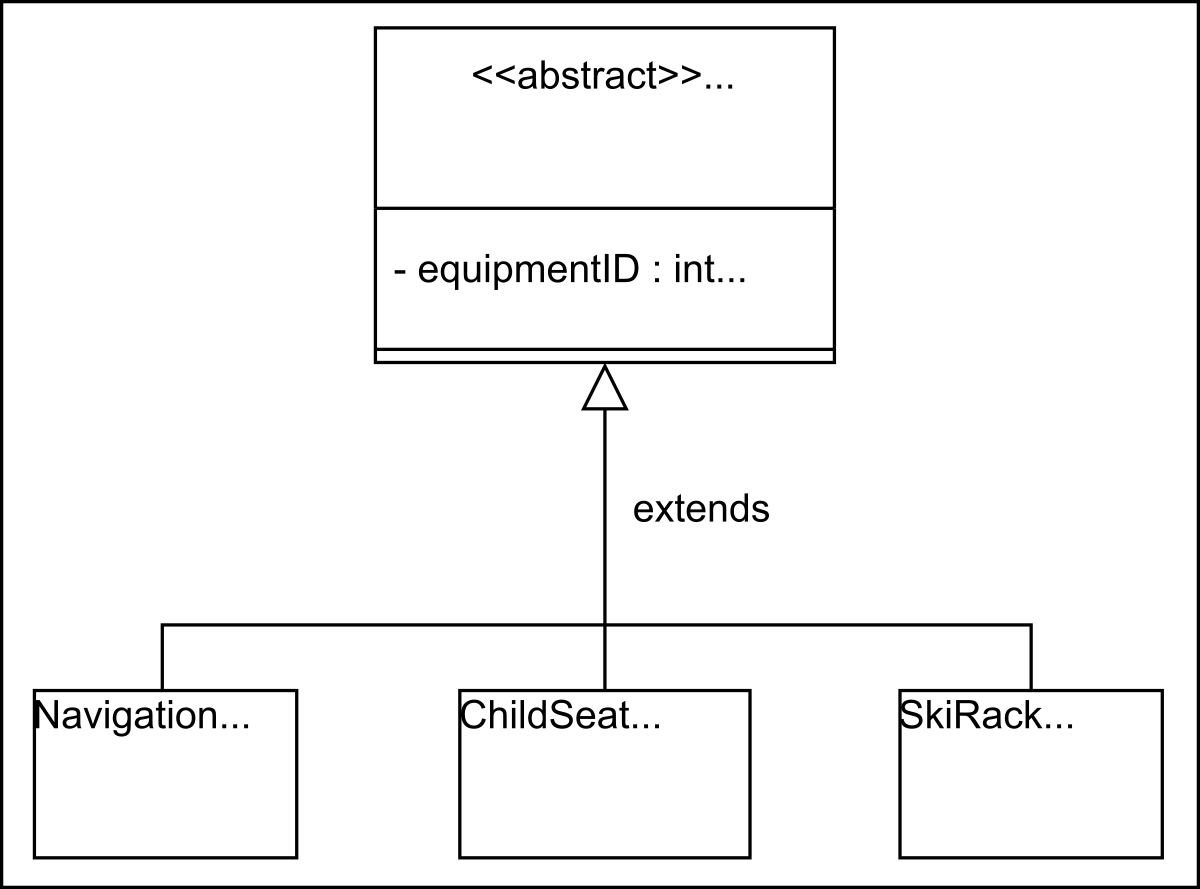
\includegraphics[width=0.5\textwidth]{Images/chapter_15/section_5607380186562560/4943337050341376.png}
 \caption{The class diagram of Equipment and its derived classes}
\end{figure}

\textbf{R8:} The system should allow the users to add equipment to the reservations, like a ski rack, child seat, and navigation.

\subsubsection{Service}\label{RaL7OUsivwIviWcLABJne-2}
\\
\texttt{Service} is an abstract class that represents the services provided to the customers along with the vehicle. While reserving a vehicle, the customers can add a service to their reservation. Every service has its fixed cost. We have three types of services, i.e., driver, roadside assistance, and Wi-Fi. The UML diagram of \texttt{Service}, along with its subclasses \texttt{DriverService}, \texttt{RoadsideAssistance}, and \texttt{Wi-Fi}, is given below:

\begin{figure}[htbp]
 \centering
 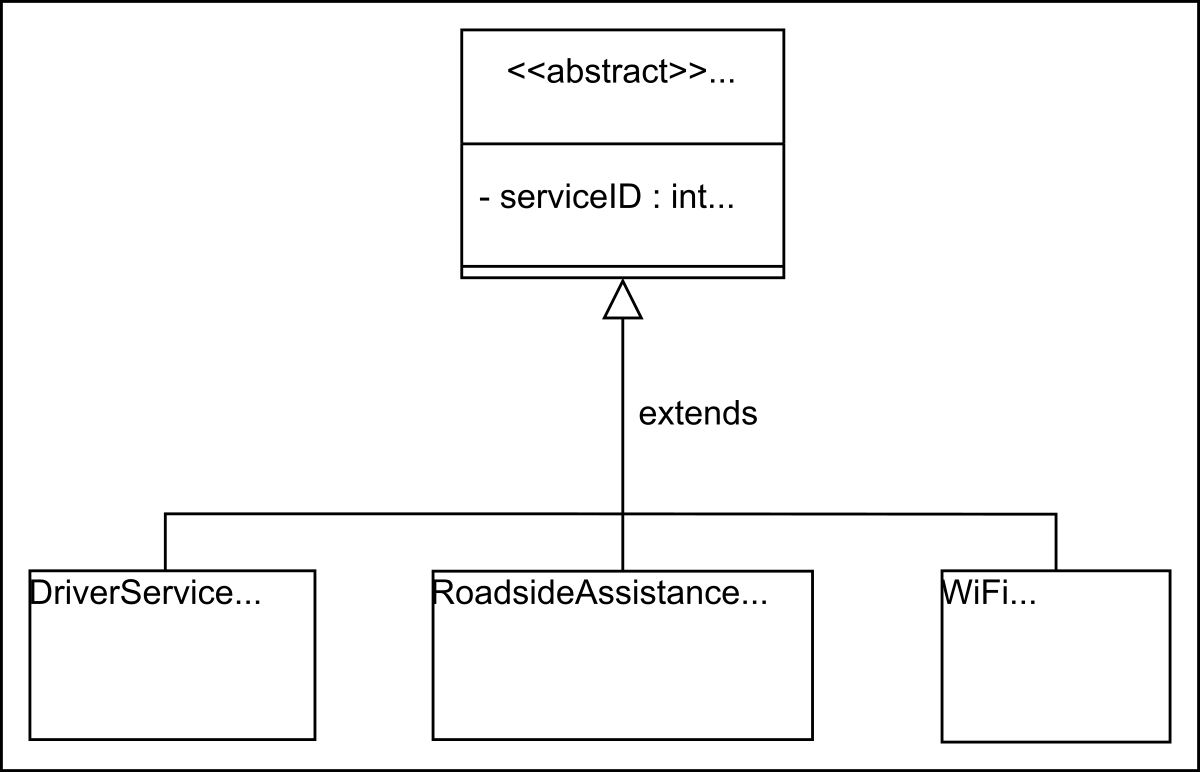
\includegraphics[width=0.5\textwidth]{Images/chapter_15/section_5607380186562560/6633653750988800.png}
 \caption{The class diagram of Service and its derived classes}
\end{figure}

\textbf{R9:} The system should allow users to add services to the reservations, like a driver, Wi-Fi, and roadside assistance.

\subsubsection{Notification}\label{FFhaZfzNUbPLfoFvRnC3-}
\\
\texttt{Notification} is an abstract class responsible for sending notifications to customers. Every notification has an ID, creation date, and content. The notification can either be an SMS notification or an email notification. The \texttt{SMSNotification} class requires the customer's phone number to send a notification, while \texttt{EmailNotification} is sent to the customer's email address. The relationship diagram of these classes is shown below:

\begin{figure}[htbp]
 \centering
 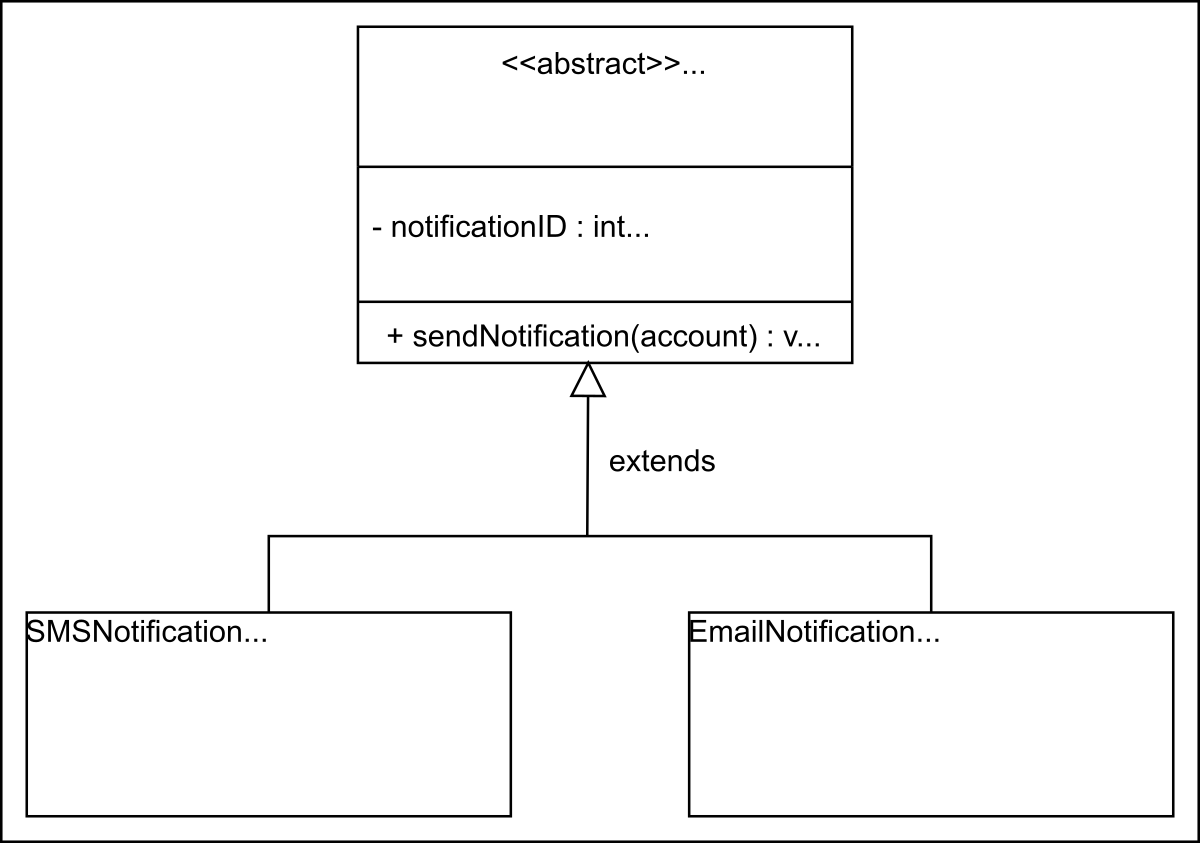
\includegraphics[width=0.5\textwidth]{Images/chapter_15/section_5607380186562560/6546235773419520.png}
 \caption{The class diagram of Notification and its derived classes}
\end{figure}

\textbf{R10:} The system should send a notification to the customer and generate a fine if the vehicle is not returned within the due date.

\subsubsection{Parking stall}\label{P4z8rT5n_HGoR9L5X9bLr-2}
\\
Each car rental location has parking stalls where the vehicles are parked. Each parking stall is identified by its ID, and a location identifier specifies its location. The representation of the \texttt{ParkingStall} class is shown below:

\begin{figure}[htbp]
 \centering
 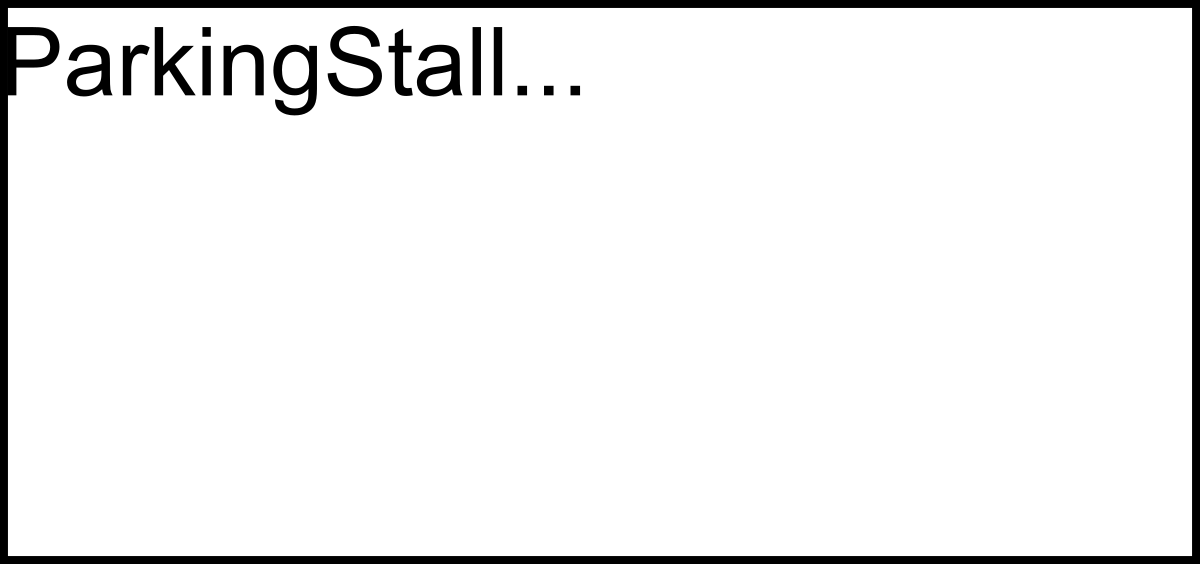
\includegraphics[width=0.5\textwidth]{Images/chapter_15/section_5607380186562560/6284891492974592.png}
 \caption{The class diagram of the ParkingStall class}
\end{figure}

\textbf{R13:} Every branch of the car rental system should have parking stalls to park the vehicles.

\subsubsection{Vehicle log}\label{P4z8rT5n_HGoR9L5X9bLr-3}
\\
\texttt{VehicleLog} is a class that is used to keep track of all the events related to a vehicle. Every vehicle log has its ID, log type, description, and creation date, as shown here:

\begin{figure}[htbp]
 \centering
 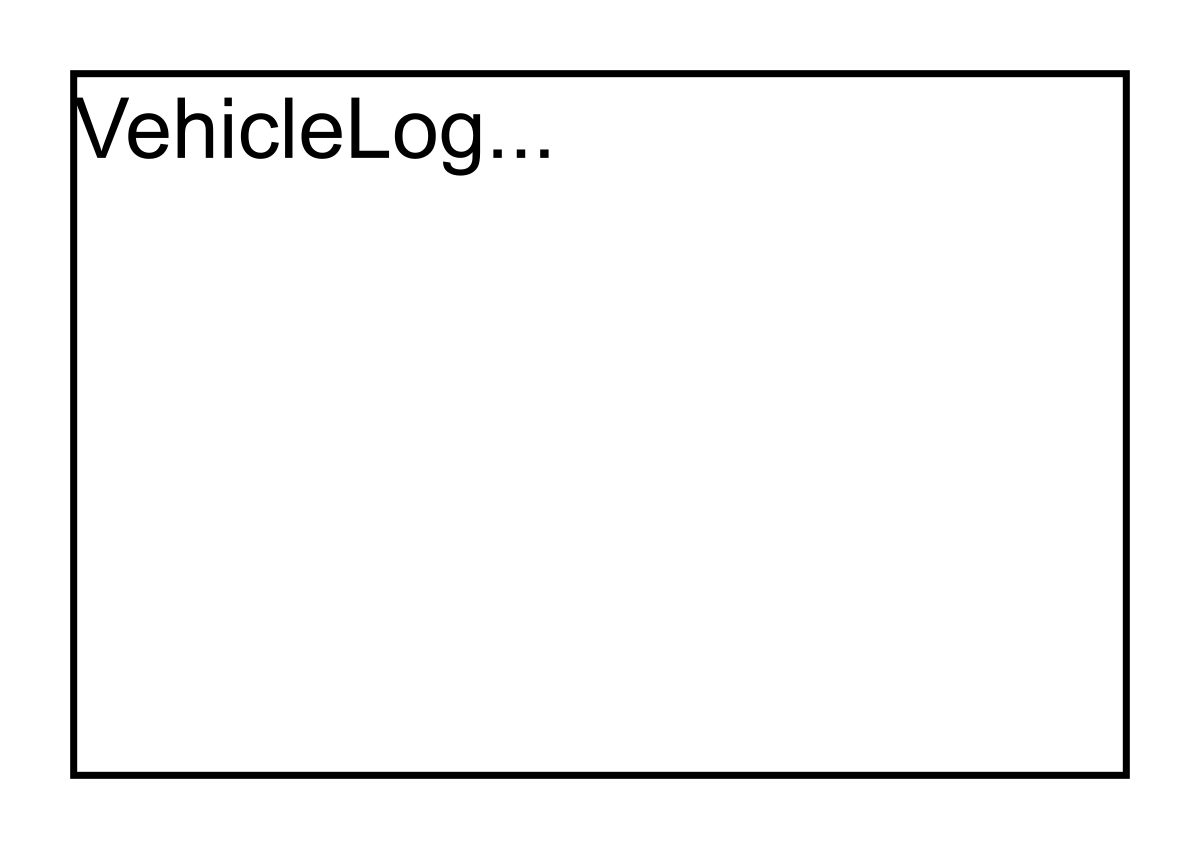
\includegraphics[width=0.5\textwidth]{Images/chapter_15/section_5607380186562560/5780484154851328.png}
 \caption{The class diagram of the VehicleLog class}
\end{figure}

\textbf{R7:} To keep track of all events related to the vehicle, the system should maintain a vehicle log.

\subsubsection{Vehicle reservation}\label{gtGnITbtcPUvC-kz2sqHI}
\\
Vehicle reservation is one of the most important requirements of the car rental system. To fulfill this functionality, we have a \texttt{VehicleReservation} class. This class is responsible for managing the vehicle reservation status of vehicles. The customer can also add any equipment or service at the time of reservation. The UML representation of the class is shown below:

\begin{figure}[htbp]
 \centering
 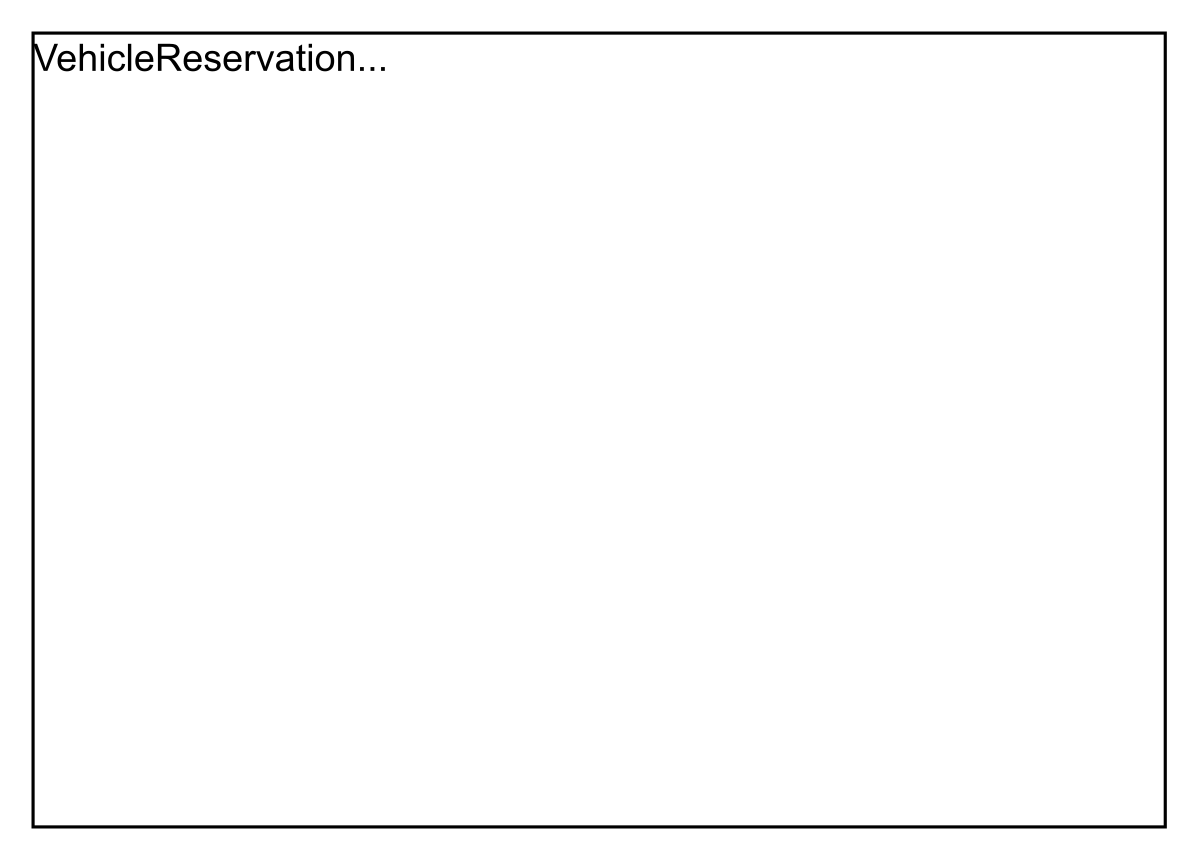
\includegraphics[width=0.5\textwidth]{Images/chapter_15/section_5607380186562560/5603252597817344.png}
 \caption{The class diagram of the VehicleReservation class}
\end{figure}

\textbf{R4:} The system should be able to keep a record of who reserved a particular vehicle and on which date the vehicle was issued.

\subsubsection{Payment}\label{f6uRomDpXqneje0s17E12-1}
\\
The \texttt{Payment} class will be an abstract class with two child classes: \texttt{CreditCard} and \texttt{Cash}. These represent the two payment methods in the car rental system. The representation of these classes is given below:

\begin{figure}[htbp]
 \centering
 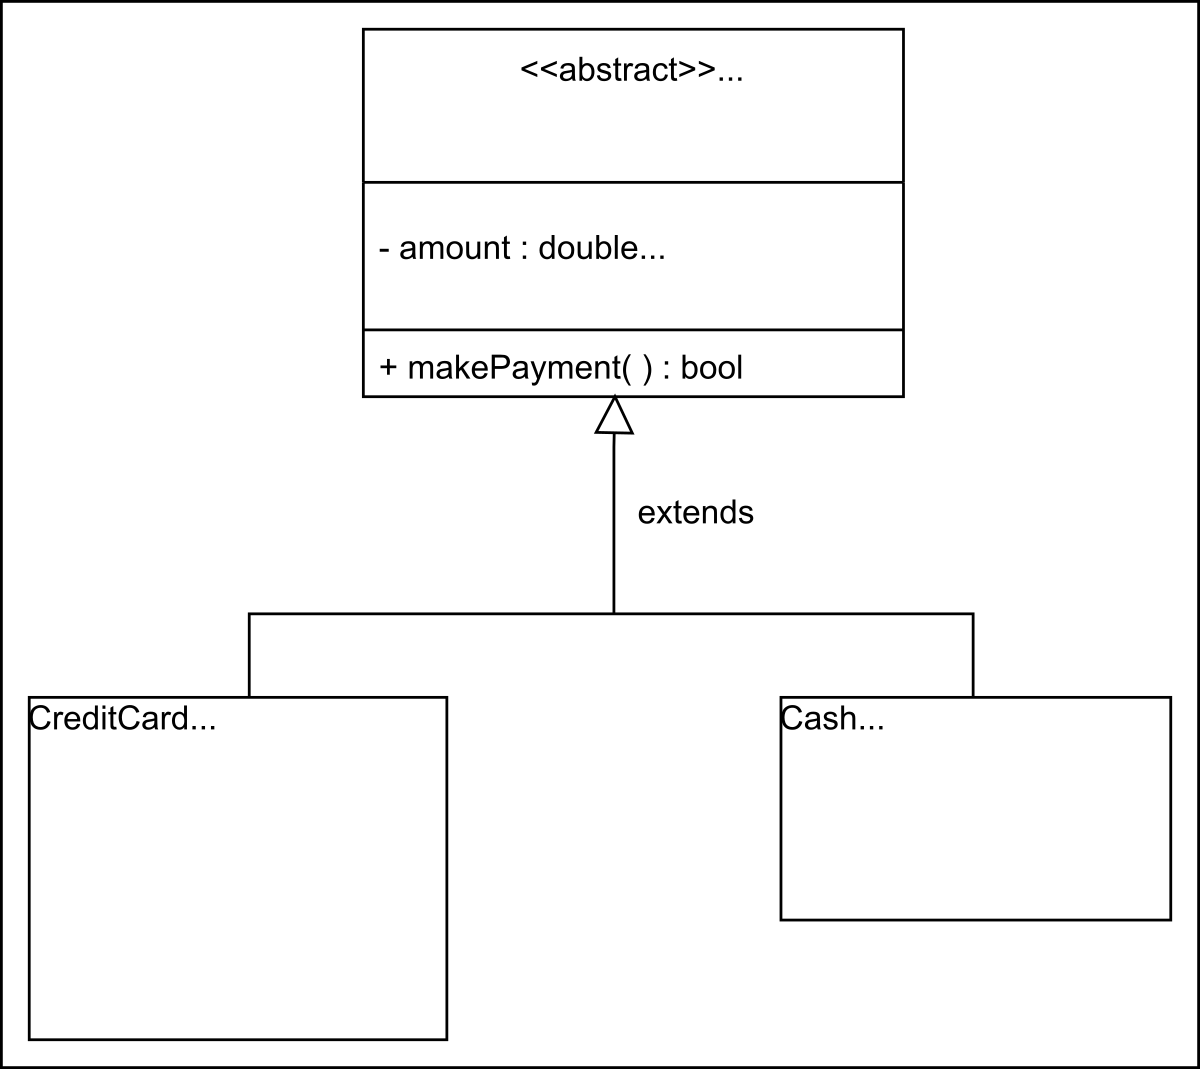
\includegraphics[width=0.5\textwidth]{Images/chapter_15/section_5607380186562560/5243244191154176.png}
 \caption{The class diagram of Payment and its child classes}
\end{figure}

\subsubsection{Fine}\label{f6uRomDpXqneje0s17E12-2}
\\
The system needs the \texttt{Fine} class to calculate the fine on the vehicle reservation in case the customer returns the vehicle after the due date, the fuel in the vehicle is less than the limit value, or there is any damage to the vehicle. The representation of this class is given below:

\begin{figure}[htbp]
 \centering
 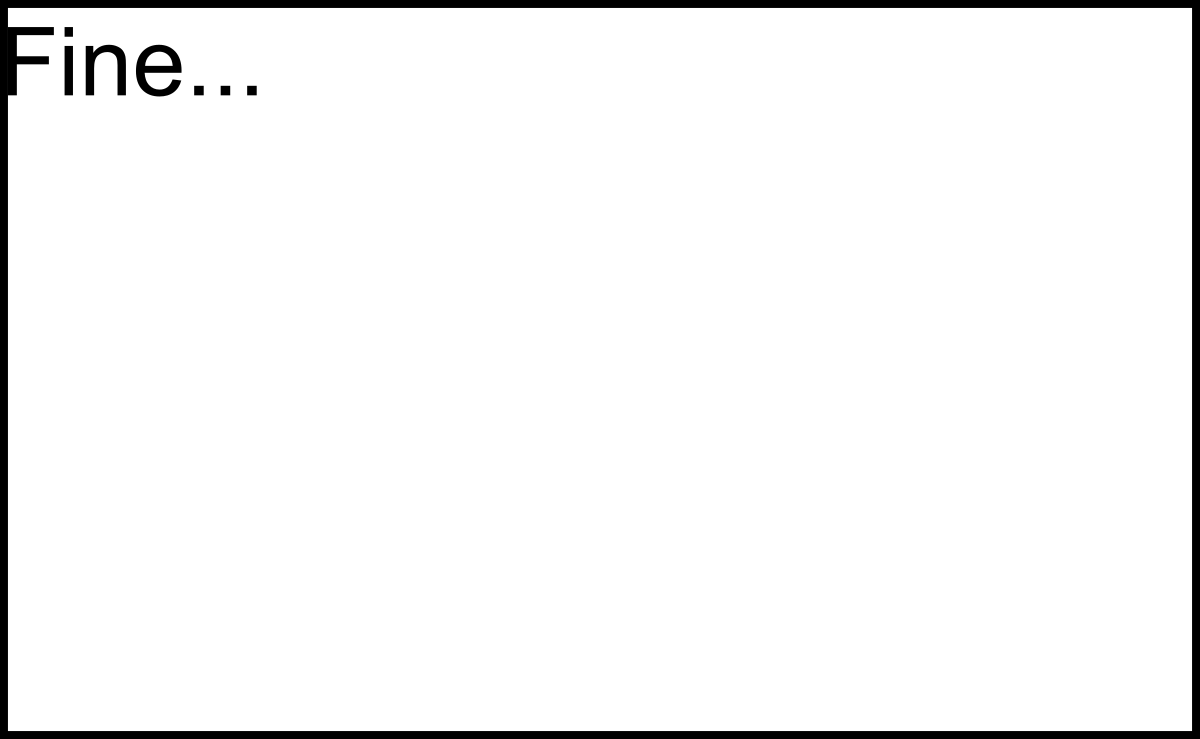
\includegraphics[width=0.5\textwidth]{Images/chapter_15/section_5607380186562560/5087804180922368.png}
 \caption{The class diagram of the Fine class}
\end{figure}

\textbf{R10:} If the vehicle is not returned by the due date, the system should send a notification to the customer and generate a fine.

\subsubsection{Search interface and vehicle inventory class}\label{U_w2glMp6e3DkE6231op0}
\\
\texttt{Search} is one of the most important functionalities of the system. It is the interface that allows the user to search for any vehicle and return the list of vehicles upon searching by any of the following methods:

\begin{itemize}
\item
\protect\phantomsection\label{4UeCVcABndVxXw80mufti}
Search for a car by its type
\item
\protect\phantomsection\label{l0tKXXVEPHDjFAz6xytw7}
Search~for a car by its model
\end{itemize}
\\
The \texttt{VehicleCatalog} is a class where the search function is implemented. In each catalog, the vehicles are sorted according to one search technique, i.e., vehicle type or model. The following UML diagram shows this relationship:

\begin{figure}[htbp]
 \centering
 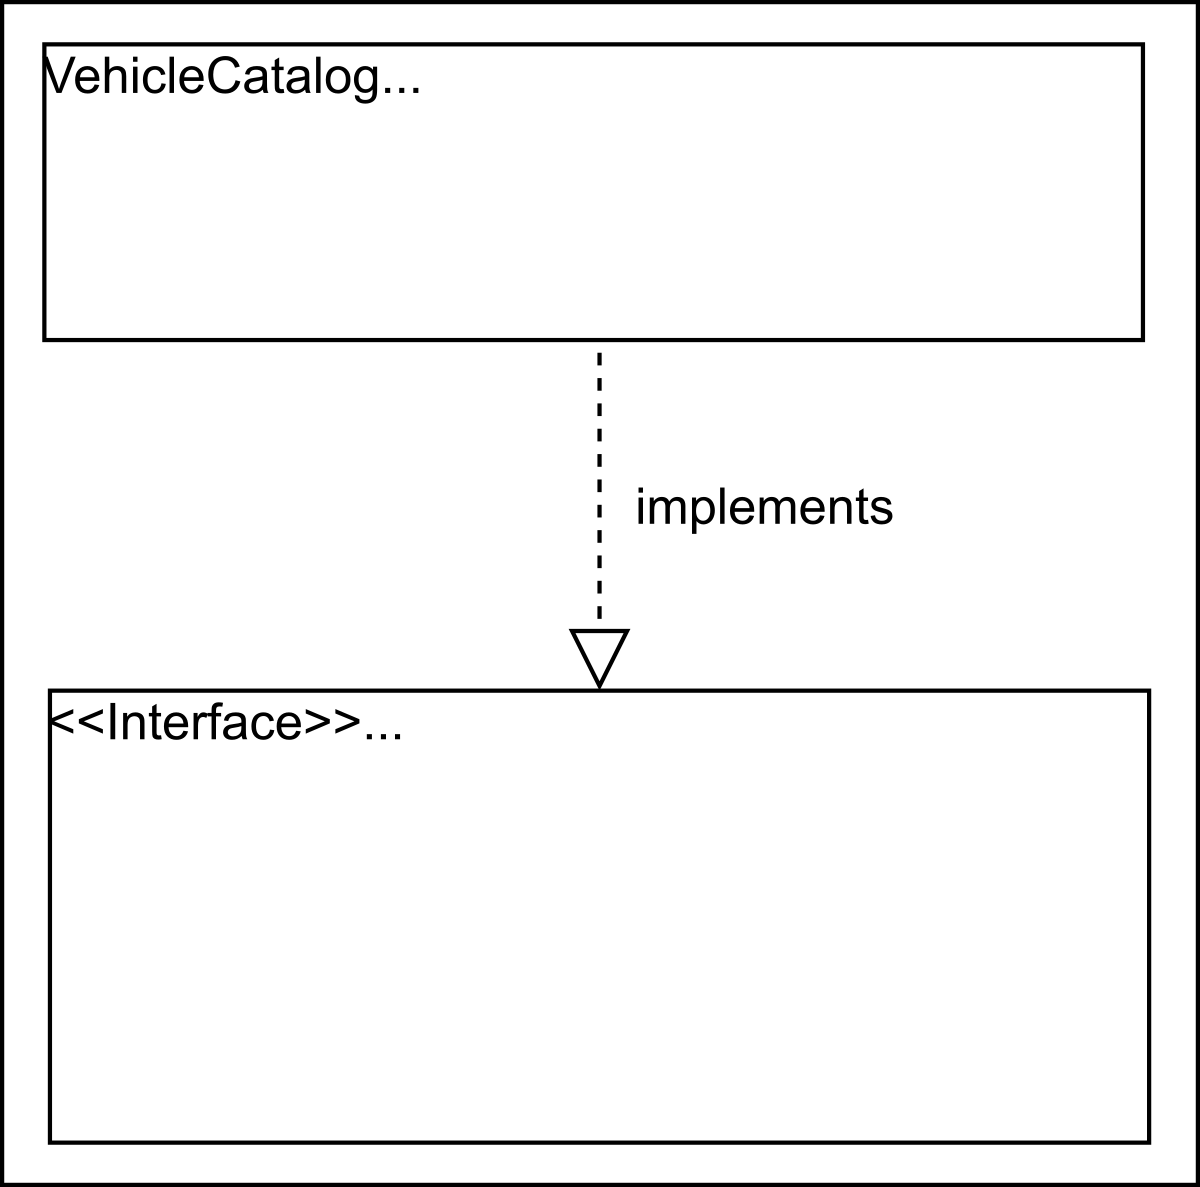
\includegraphics[width=0.5\textwidth]{Images/chapter_15/section_5607380186562560/5666020649074688.png}
 \caption{The class diagram of the Search interface and the VehicleCatalog class}
\end{figure}

\textbf{R11:} The system should allow users to search vehicles by type, model, or seat capacity.

\subsubsection{Car rental system and branch}\label{G3lnGUGzNztdMf7PxzK75}
\\
\texttt{CarRentalSystem} is the main class of the car rental system and is the central part of the design. There can be multiple branches and locations of the car rental system. The \texttt{CarRentalBranch} class will represent each of these branches. The class representation is as follows:

\begin{figure}[htbp]
 \centering
 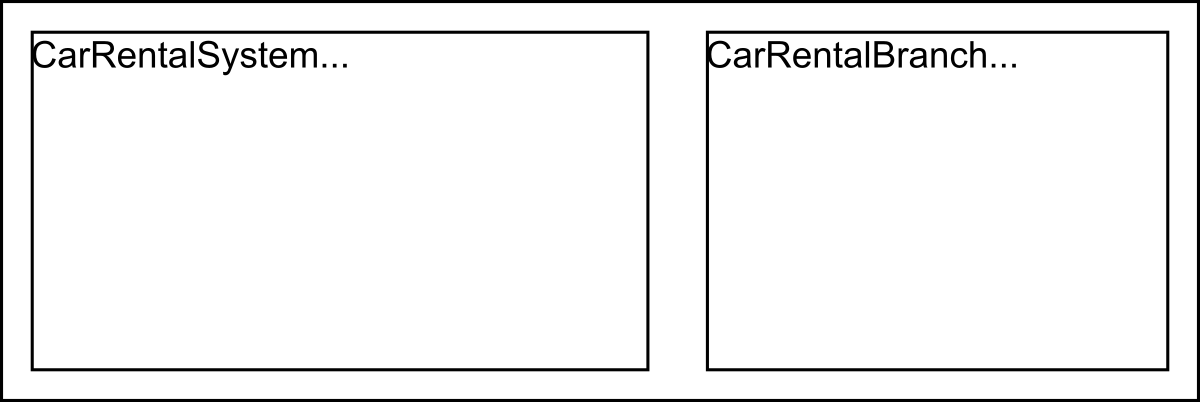
\includegraphics[width=0.5\textwidth]{Images/chapter_15/section_5607380186562560/6175400045838336.png}
 \caption{The class diagram of the CarRentalSystem and CarRentalBranch classes}
\end{figure}

\textbf{R12:} A system should be able to manage the multiple branches of the car rental system.

\subsubsection{Enumerations}\label{unp3y-QDa6psC3OH52thY-2}
\\
The list of enumerations required in the car rental system is provided below:

\begin{itemize}
\item
\protect\phantomsection\label{L7Q4_d--pCzFdvsuSYz9G}
\textbf{\texttt{VehicleStatus}:} The vehicle status describes the status of the particular vehicle for the user, whether it is available, reserved, lost, or serviced.
\item
\protect\phantomsection\label{J3Mj7FmXUAJUtL10XBcrY}
\textbf{\texttt{AccountStatus}:} The account status tells about the user account status, i.e., active, closed, canceled, banned, or blocked.
\item
\protect\phantomsection\label{MLKloIqzHmWNOso64XpKK}
\textbf{\texttt{ReservationStatus}:} The reservation status tells about the reservation state of any vehicle, whether it is in an active state, pending state, confirmed state, completed state, or canceled state.
\item
\protect\phantomsection\label{9R5vDWLJ3eFdh9YPLb5QL}
\textbf{\texttt{PaymentStatus}:} The payment status checks if the customer's payment falls in any of the following stages: unpaid, pending, completed, canceled, or refunded.
\item
\protect\phantomsection\label{zdp2ZvpuWCZVhqQm8xlND}
\textbf{\texttt{VanType}:} The van type specifies that it can only be of two types: passenger or cargo.
\item
\protect\phantomsection\label{NWXwlsVfKwYDtK0gGv68p}
\textbf{\texttt{CarType}:} The car type describes the different types of cars, whether they are economy, compact, intermediate, standard, full-size, premium, or luxury.
\item
\protect\phantomsection\label{pyxfocYUg7Y6A1WtyGoEq}
\textbf{\texttt{MotorcycleType}:} Similar to the car type, the motorcycle type describes the different types of motorcycles, whether standard, cruiser, touring, sports, off-road, or dual-purpose.
\item
\protect\phantomsection\label{xtFuQkqwtVU0_jWg9cz5F}
\textbf{\texttt{TruckType}:} The truck type specifies whether the truck is light-duty, medium-duty, or heavy-duty.
\item
\protect\phantomsection\label{_MxNjZt9g6Ae8E30ySwJQ}
\textbf{\texttt{VehicleLogType}:} The vehicle log type describes the type of a particular vehicle log, whether it is an accident, fueling, cleaning service, oil change, repair, or other.
\end{itemize}
\\
These enumerations can be represented using the following class diagram:

\begin{figure}[htbp]
 \centering
 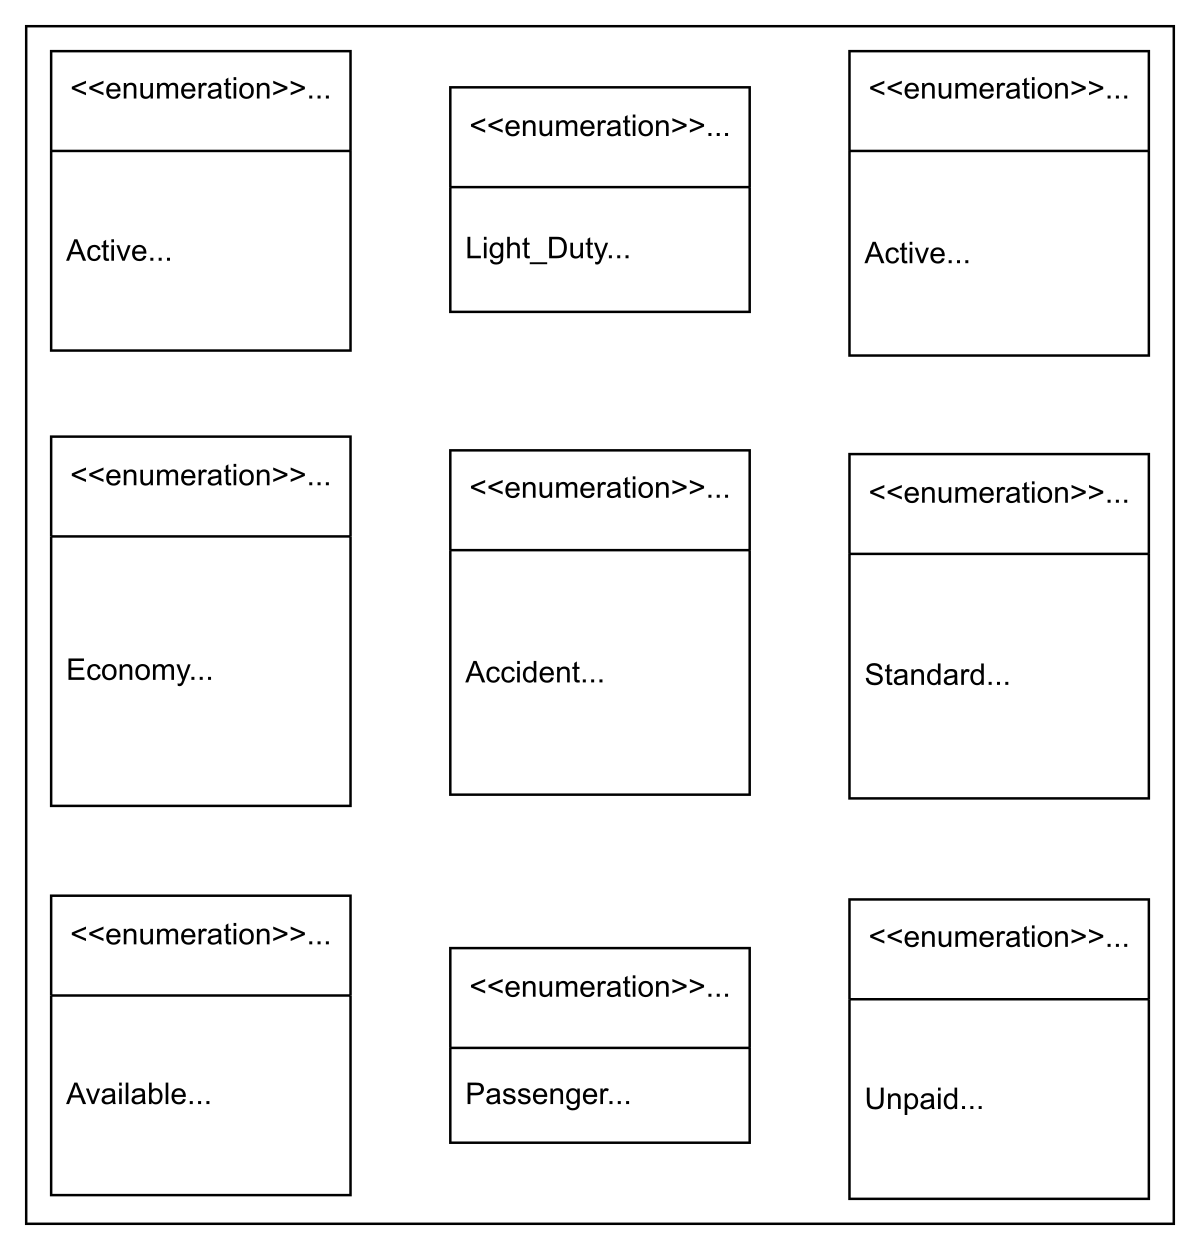
\includegraphics[width=0.5\textwidth]{Images/chapter_15/section_5607380186562560/6599176962834432.png}
 \caption{Enums in the car rental system}
\end{figure}

\textbf{R3:} Vehicles can have multiple subtypes. The car type can be economy, luxury, standard, or compact. The van type can be passenger or cargo type. Moreover, the motorcycle type can be cruiser, touring, or sports. The truck type can be light, medium, or high-duty.

\subsection{Relationship between the classes}\label{TQeQvn7wVlq23DuZpRwW7}
\\
Now, let's discuss the relationships between the main classes in our Car Rental System. Understanding these relationships helps us design for maintainability, extensibility, and clarity.

\subsubsection{Association}\label{3fdYzSgUg79AkbbTibie1}
\\
Association represents a ``uses'' or ``knows about'' relationship between two classes. The class diagram will have the following association relationships:

\begin{itemize}
\item
\protect\phantomsection\label{1QvMk1LavXtUjagkVz5O1}
\textbf{One-way association:}

\begin{itemize}
\item
The \texttt{Account} class should have a one-way association with the \texttt{VehicleReservation} class.
\item
The \texttt{VehicleReservation} class will have a one-way association with the \texttt{Vehicle} class. This means they reference \texttt{Vehicle} (e.g., by storing a vehicle ID or a reference), but \texttt{Vehicle} does not reference them back.
\item
The \texttt{Fine} class has a one-way association with \texttt{Payment}, as a fine is calculated based on or linked to a specific payment, but payment does not necessarily reference a fine.
\end{itemize}
\end{itemize}

\begin{figure}[htbp]
 \centering
 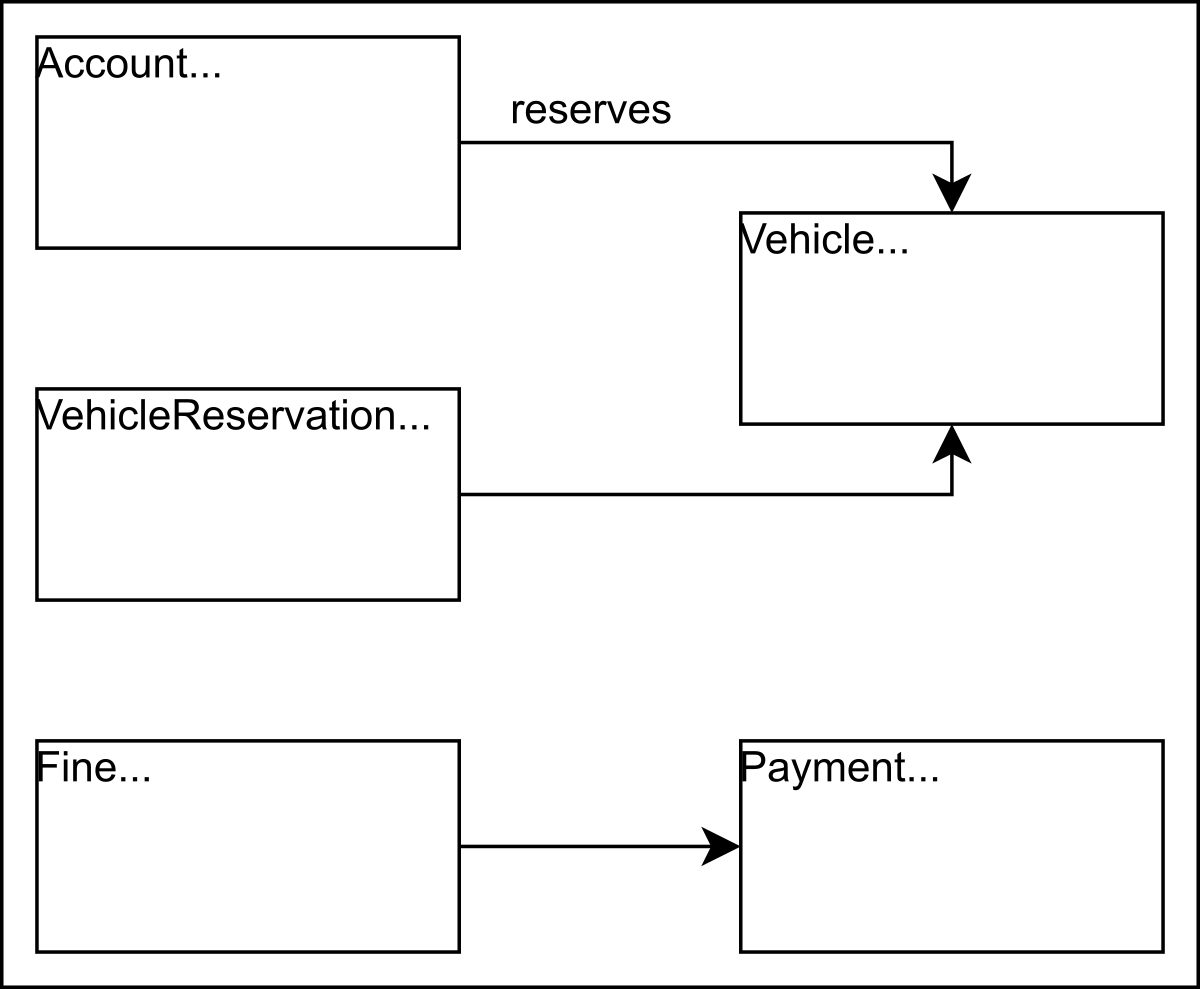
\includegraphics[width=0.5\textwidth]{Images/chapter_15/section_5607380186562560/4792159687671808.png}
 \caption{The one-way association relationship between classes}
\end{figure}

\begin{itemize}
\item
\protect\phantomsection\label{QuSjXa91e44O_cJj99Rwj}
\textbf{Two-way association:}

\begin{itemize}
\item
The \texttt{VehicleReservation} class has a two-way association with both \texttt{Payment} and \texttt{Notification}. A reservation is linked to payment(s) and notifications (for confirmation, reminders, etc.), and payments/notifications can also reference the associated reservation if needed.
\end{itemize}
\end{itemize}

\begin{figure}[htbp]
 \centering
 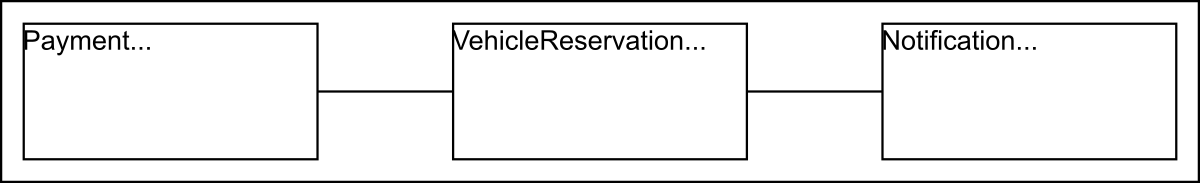
\includegraphics[width=0.5\textwidth]{Images/chapter_15/section_5607380186562560/4861392949870592.png}
 \caption{The two-way association relationship between classes}
\end{figure}

\subsubsection{Composition}\label{GrRDd34coTgbIpqCD8jOl-1}
\\
Composition represents a strong ``has-a'' relationship, where the lifetime of the part is controlled by the whole. The class diagram will have the following composition relationships:

\begin{itemize}
\item
\protect\phantomsection\label{f-Fb-4iN5Qq41mU5xTSrm}
The \texttt{CarRentalBranch} class is composed of multiple \texttt{ParkingStall} instances. If the branch is deleted, its parking stalls cease to exist.
\item
\protect\phantomsection\label{bV-JOPAWhiQwY1BnqpCBc}
The \texttt{Vehicle} class is composed of \texttt{VehicleLog} entries. Logs exist only as long as the vehicle exists.
\end{itemize}

\begin{figure}[htbp]
 \centering
 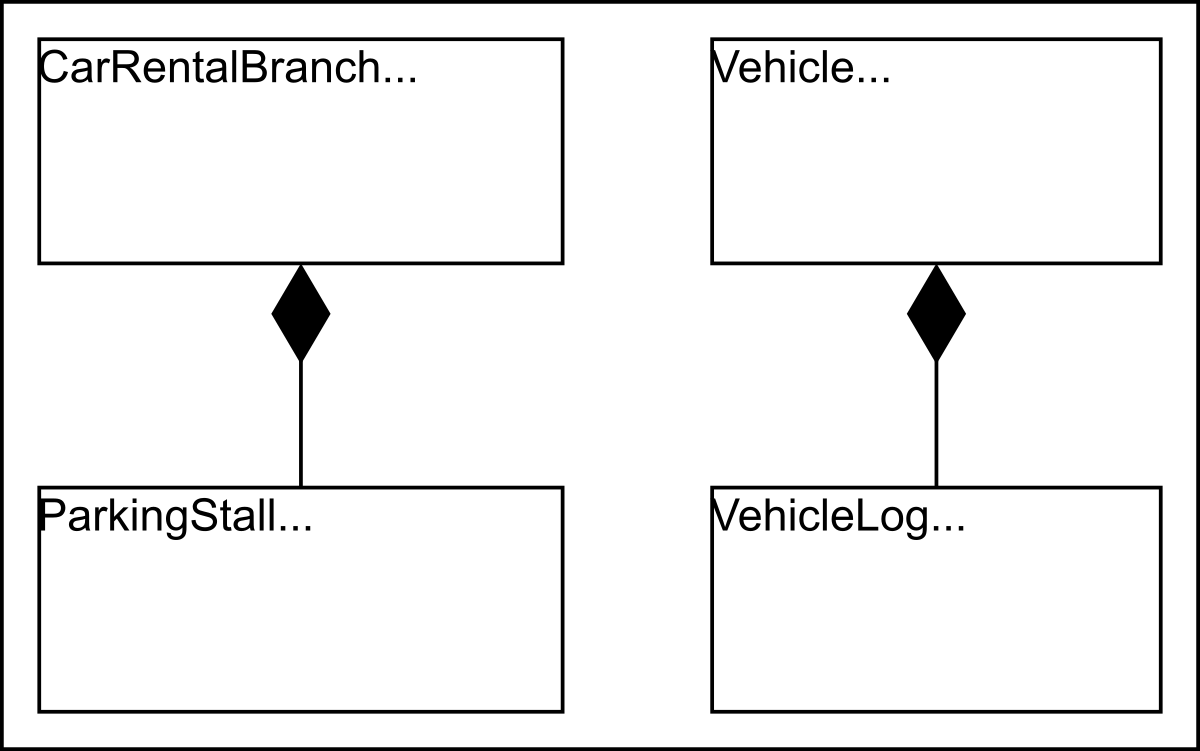
\includegraphics[width=0.5\textwidth]{Images/chapter_15/section_5607380186562560/6326941655498752.png}
 \caption{The composition relationship between classes}
\end{figure}

\subsubsection{Aggregation}\label{GrRDd34coTgbIpqCD8jOl-2}
\\
Aggregation is a weaker ``has-a'' relationship, where the part can exist independently of the whole. The following classes show an aggregation relationship:

\begin{itemize}
\item
\protect\phantomsection\label{-LB4i9scW31KIU2QnAjLh}
The \texttt{CarRentalSystem} class aggregates multiple \texttt{CarRentalBranch} instances, meaning branches can exist independently and could potentially be shared or moved between systems.
\item
\protect\phantomsection\label{Fy8Xbe4aKeCXuvLeR52Rt}
The \texttt{ParkingStall} and \texttt{VehicleCatalog} classes aggregate \texttt{Vehicle} instances; a vehicle can be reassigned or exist elsewhere.
\item
\protect\phantomsection\label{lfijQNxZhHotRBQ7rDGvK}
The \texttt{VehicleReservation} class aggregates multiple \texttt{Equipment} and \texttt{Service} instances; equipment and services can be reused across reservations or elsewhere in the system.
\end{itemize}

\begin{figure}[htbp]
 \centering
 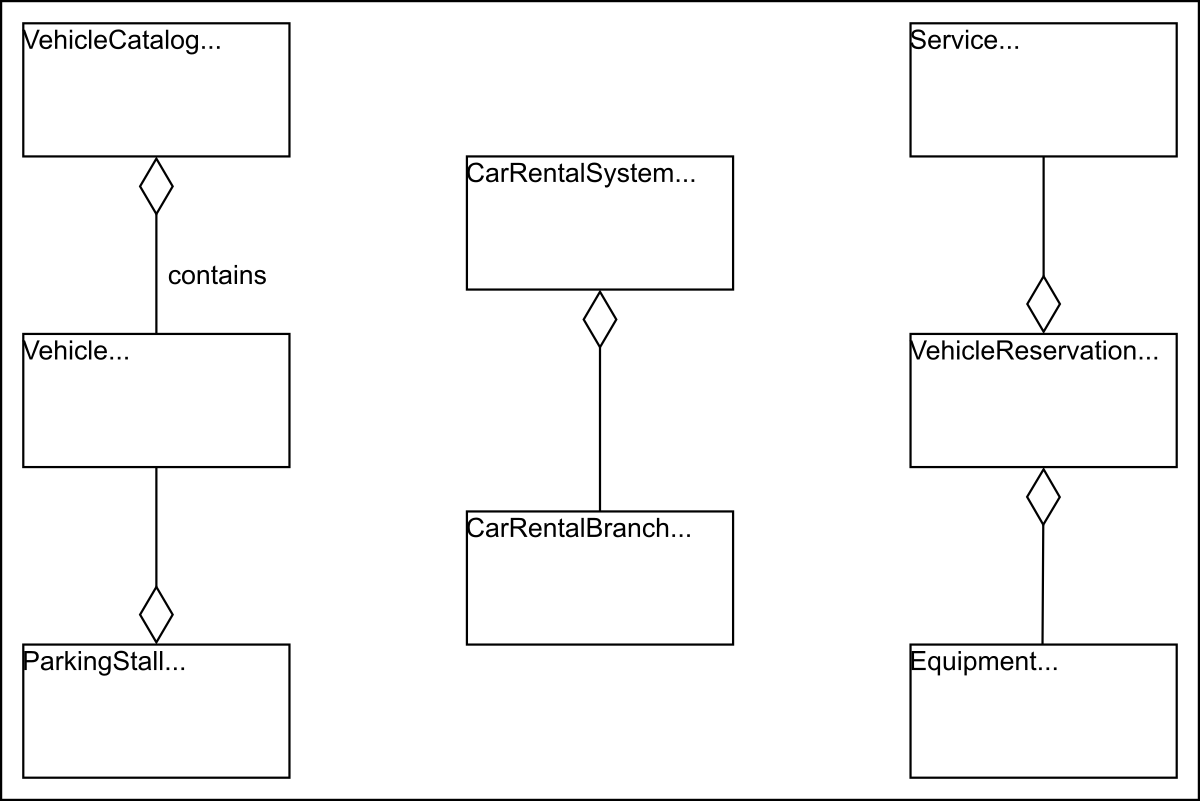
\includegraphics[width=0.5\textwidth]{Images/chapter_15/section_5607380186562560/4806615155081216.png}
 \caption{The aggregation relationship between classes}
\end{figure}

\subsubsection{Inheritance}\label{MR1f3aHJk_bB1LITZLBgq}
\\
Inheritance represents an ``is-a'' relationship. The following classes show an inheritance relationship:

\begin{itemize}
\item
\protect\phantomsection\label{eMLSVsxglKiuW1-9Gb6jN}
The \texttt{Receptionist} and \texttt{Customer} classes extend the abstract \texttt{Account} class, inheriting its fields and methods.
\item
\protect\phantomsection\label{XhTko1FXHZ30Xvm4ePPG1}
The \texttt{Account} class extends the \texttt{Person} class, inheriting personal information.
\item
\protect\phantomsection\label{20lcnkQ4r2GN6kfi64JdO}
The \texttt{Car}, \texttt{Truck}, \texttt{Van}, and \texttt{Motorcycle} classes extend the \texttt{Vehicle} class, each representing a specialized vehicle type.
\item
\protect\phantomsection\label{Bq210yt1H3Vrm-ZK7Ocvu}
The \texttt{DriverService}, \texttt{RoadsideAssistance}, and \texttt{WiFi} classes extend the abstract \texttt{Service} class.
\item
\protect\phantomsection\label{REVZGHh4V5ctLUMXKk-oZ}
The \texttt{Navigation}, \texttt{ChildSeat}, and \texttt{SkiRack} classes extend the abstract \texttt{Equipment} class.
\item
\protect\phantomsection\label{njQ0fThg5CfJapc_WU9lU}
The \texttt{SmsNotification} and \texttt{EmailNotification} classes extend the abstract \texttt{Notification} class.
\item
\protect\phantomsection\label{8ivbpoXYyh13KXBb-uWxt}
The \texttt{Cash} and \texttt{CreditCard} classes extend the abstract \texttt{Payment} class.
\item
\protect\phantomsection\label{mjLGZ03SSFkMPMmccqhsW}
The \texttt{VehicleCatalog} class implements the \texttt{Search} interface, enabling searching for vehicles by type or model.
\end{itemize}

\begin{figure}[htbp]
 \centering
 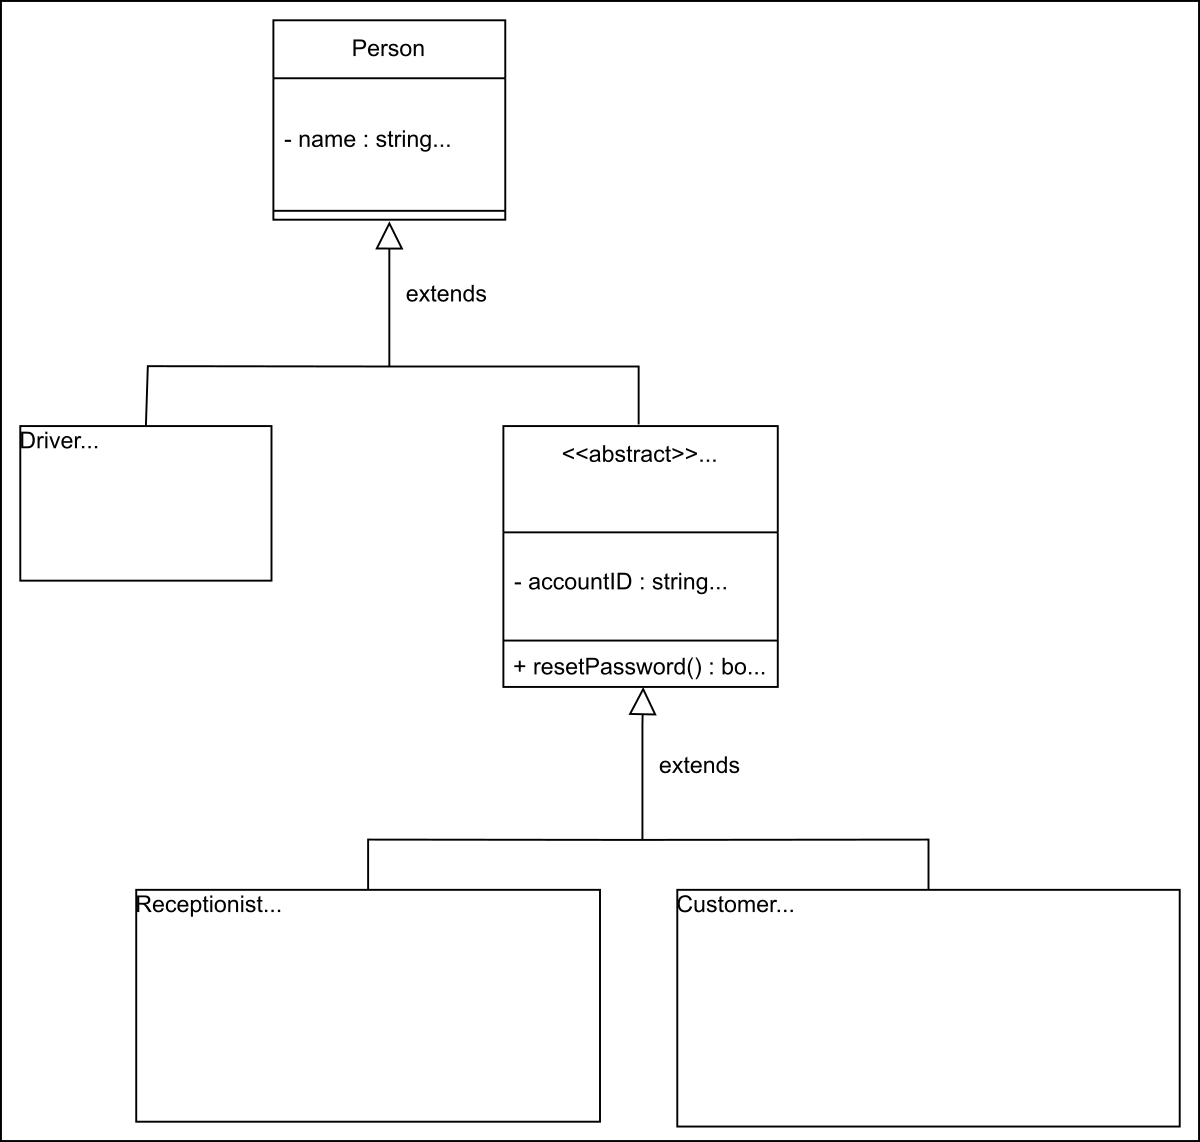
\includegraphics[width=0.5\textwidth]{Images/chapter_15/section_5607380186562560/4818710406889472.png}
 \caption{The class diagram of the different users of our system}
\end{figure}

\begin{quote}
\textbf{Note:} We've already discussed the inheritance relationship between classes in the component section above one by one.
\end{quote}
\subsection{Class diagram of the car rental system}\label{kTQNSNPtrG90Q1J91scMn}
\\
This section outlines the multiplicity (cardinality) relationships between the main classes in our car rental system. For each relationship, we explain the allowed number of instances on each side and the real-world or design rationale behind the connection. Understanding these relationships is key to modeling how different entities interact and collaborate to support key workflows in the system.

\begin{center}
{\def\LTcaptype{none} % do not increment counter
\begin{longtable}[]{@{}
>{\raggedright\arraybackslash} p{(\linewidth - 6\tabcolsep) * \real{0.2500}}
>{\raggedright\arraybackslash} p{(\linewidth - 6\tabcolsep) * \real{0.2500}}
>{\raggedright\arraybackslash} p{(\linewidth - 6\tabcolsep) * \real{0.2500}}
>{\raggedright\arraybackslash} p{(\linewidth - 6\tabcolsep) * \real{0.2500}}@{}}
\toprule\noalign{}
\endhead
\bottomrule\noalign{}
\endlastfoot
\begin{minipage}[t]{\linewidth}\raggedright
\textbf{Source}
\end{minipage} & \begin{minipage}[t]{\linewidth}\raggedright
\textbf{Target}
\end{minipage} & \begin{minipage}[t]{\linewidth}\raggedright
\textbf{Multiplicity}
\end{minipage} & \begin{minipage}[t]{\linewidth}\raggedright
\textbf{Reason}
\end{minipage} \\
\begin{minipage}[t]{\linewidth}\raggedright
\texttt{CarRentalSystem}
\end{minipage} & \begin{minipage}[t]{\linewidth}\raggedright
\texttt{CarRentalBranch}
\end{minipage} & \begin{minipage}[t]{\linewidth}\raggedright
1-\/-0..*
\end{minipage} & \begin{minipage}[t]{\linewidth}\raggedright
A car rental system manages zero or more branches (locations).
\end{minipage} \\
\begin{minipage}[t]{\linewidth}\raggedright
\texttt{CarRentalBranch}
\end{minipage} & \begin{minipage}[t]{\linewidth}\raggedright
\texttt{ParkingStall}
\end{minipage} & \begin{minipage}[t]{\linewidth}\raggedright
1-\/-0..*
\end{minipage} & \begin{minipage}[t]{\linewidth}\raggedright
Each branch consists of multiple parking stalls where vehicles are parked.
\end{minipage} \\
\begin{minipage}[t]{\linewidth}\raggedright
\texttt{ParkingStall}
\end{minipage} & \begin{minipage}[t]{\linewidth}\raggedright
\texttt{Vehicle}
\end{minipage} & \begin{minipage}[t]{\linewidth}\raggedright
0..*-\/-1
\end{minipage} & \begin{minipage}[t]{\linewidth}\raggedright
Each parking stall can hold one vehicle, but a vehicle could move between stalls; the diagram shows composition at the branch-level, so each stall is unique.
\end{minipage} \\
\begin{minipage}[t]{\linewidth}\raggedright
\texttt{Vehicle}
\end{minipage} & \begin{minipage}[t]{\linewidth}\raggedright
\texttt{VehicleLog}
\end{minipage} & \begin{minipage}[t]{\linewidth}\raggedright
1-\/-0..*
\end{minipage} & \begin{minipage}[t]{\linewidth}\raggedright
Each vehicle has zero or more logs to track events (accidents, maintenance, etc.).
\end{minipage} \\
\begin{minipage}[t]{\linewidth}\raggedright
\texttt{VehicleCatalog}
\end{minipage} & \begin{minipage}[t]{\linewidth}\raggedright
\texttt{Vehicle}
\end{minipage} & \begin{minipage}[t]{\linewidth}\raggedright
1-\/-0..*
\end{minipage} & \begin{minipage}[t]{\linewidth}\raggedright
The catalog contains references to all available vehicles for searching.
\end{minipage} \\
\begin{minipage}[t]{\linewidth}\raggedright
\texttt{VehicleReservation}
\end{minipage} & \begin{minipage}[t]{\linewidth}\raggedright
\texttt{Vehicle}
\end{minipage} & \begin{minipage}[t]{\linewidth}\raggedright
1-\/-1
\end{minipage} & \begin{minipage}[t]{\linewidth}\raggedright
Each reservation is associated with exactly one vehicle.
\end{minipage} \\
\begin{minipage}[t]{\linewidth}\raggedright
\texttt{VehicleReservation}
\end{minipage} & \begin{minipage}[t]{\linewidth}\raggedright
\texttt{Account}
\end{minipage} & \begin{minipage}[t]{\linewidth}\raggedright
0..*-\/-1
\end{minipage} & \begin{minipage}[t]{\linewidth}\raggedright
One customer makes each reservation, but a customer may have multiple reservations (not shown by the arrow but reflected in the code).
\end{minipage} \\
\begin{minipage}[t]{\linewidth}\raggedright
\texttt{VehicleReservation}
\end{minipage} & \begin{minipage}[t]{\linewidth}\raggedright
\texttt{Equipment}
\end{minipage} & \begin{minipage}[t]{\linewidth}\raggedright
1-\/-0..*
\end{minipage} & \begin{minipage}[t]{\linewidth}\raggedright
Each reservation can include zero or more equipment (child seat, ski rack, etc.).
\end{minipage} \\
\begin{minipage}[t]{\linewidth}\raggedright
\texttt{VehicleReservation}
\end{minipage} & \begin{minipage}[t]{\linewidth}\raggedright
\texttt{Service}
\end{minipage} & \begin{minipage}[t]{\linewidth}\raggedright
1-\/-0..*
\end{minipage} & \begin{minipage}[t]{\linewidth}\raggedright
Each reservation can include zero or more optional services (WiFi, driver, roadside assistance).
\end{minipage} \\
\begin{minipage}[t]{\linewidth}\raggedright
\texttt{VehicleReservation}
\end{minipage} & \begin{minipage}[t]{\linewidth}\raggedright
\texttt{Payment}
\end{minipage} & \begin{minipage}[t]{\linewidth}\raggedright
1-\/-1
\end{minipage} & \begin{minipage}[t]{\linewidth}\raggedright
Each reservation involves exactly one payment.
\end{minipage} \\
\begin{minipage}[t]{\linewidth}\raggedright
\texttt{VehicleReservation}
\end{minipage} & \begin{minipage}[t]{\linewidth}\raggedright
\texttt{Notification}
\end{minipage} & \begin{minipage}[t]{\linewidth}\raggedright
1-\/-0..*
\end{minipage} & \begin{minipage}[t]{\linewidth}\raggedright
Each reservation can result in zero or more notifications (confirmation, cancellation, etc.).
\end{minipage} \\
\begin{minipage}[t]{\linewidth}\raggedright
\texttt{Fine}
\end{minipage} & \begin{minipage}[t]{\linewidth}\raggedright
\texttt{Payment}
\end{minipage} & \begin{minipage}[t]{\linewidth}\raggedright
0..1-\/-1
\end{minipage} & \begin{minipage}[t]{\linewidth}\raggedright
A fine is linked to one payment (if incurred), but not all payments result from fines.
\end{minipage} \\
\begin{minipage}[t]{\linewidth}\raggedright
\texttt{Customer}
\end{minipage} & \begin{minipage}[t]{\linewidth}\raggedright
\texttt{Account}
\end{minipage} & \begin{minipage}[t]{\linewidth}\raggedright
1-\/-1
\end{minipage} & \begin{minipage}[t]{\linewidth}\raggedright
Each customer is an account.
\end{minipage} \\
\begin{minipage}[t]{\linewidth}\raggedright
\texttt{Receptionist}
\end{minipage} & \begin{minipage}[t]{\linewidth}\raggedright
\texttt{Account}
\end{minipage} & \begin{minipage}[t]{\linewidth}\raggedright
1-\/-1
\end{minipage} & \begin{minipage}[t]{\linewidth}\raggedright
Each receptionist is an account.
\end{minipage} \\
\begin{minipage}[t]{\linewidth}\raggedright
\texttt{Account}
\end{minipage} & \begin{minipage}[t]{\linewidth}\raggedright
\texttt{Person}
\end{minipage} & \begin{minipage}[t]{\linewidth}\raggedright
1-\/-1
\end{minipage} & \begin{minipage}[t]{\linewidth}\raggedright
Each account corresponds to a person with contact information.
\end{minipage} \\
\end{longtable}
}
\end{center}

Here's the class diagram of the car rental system:

\begin{figure}[htbp]
 \centering
 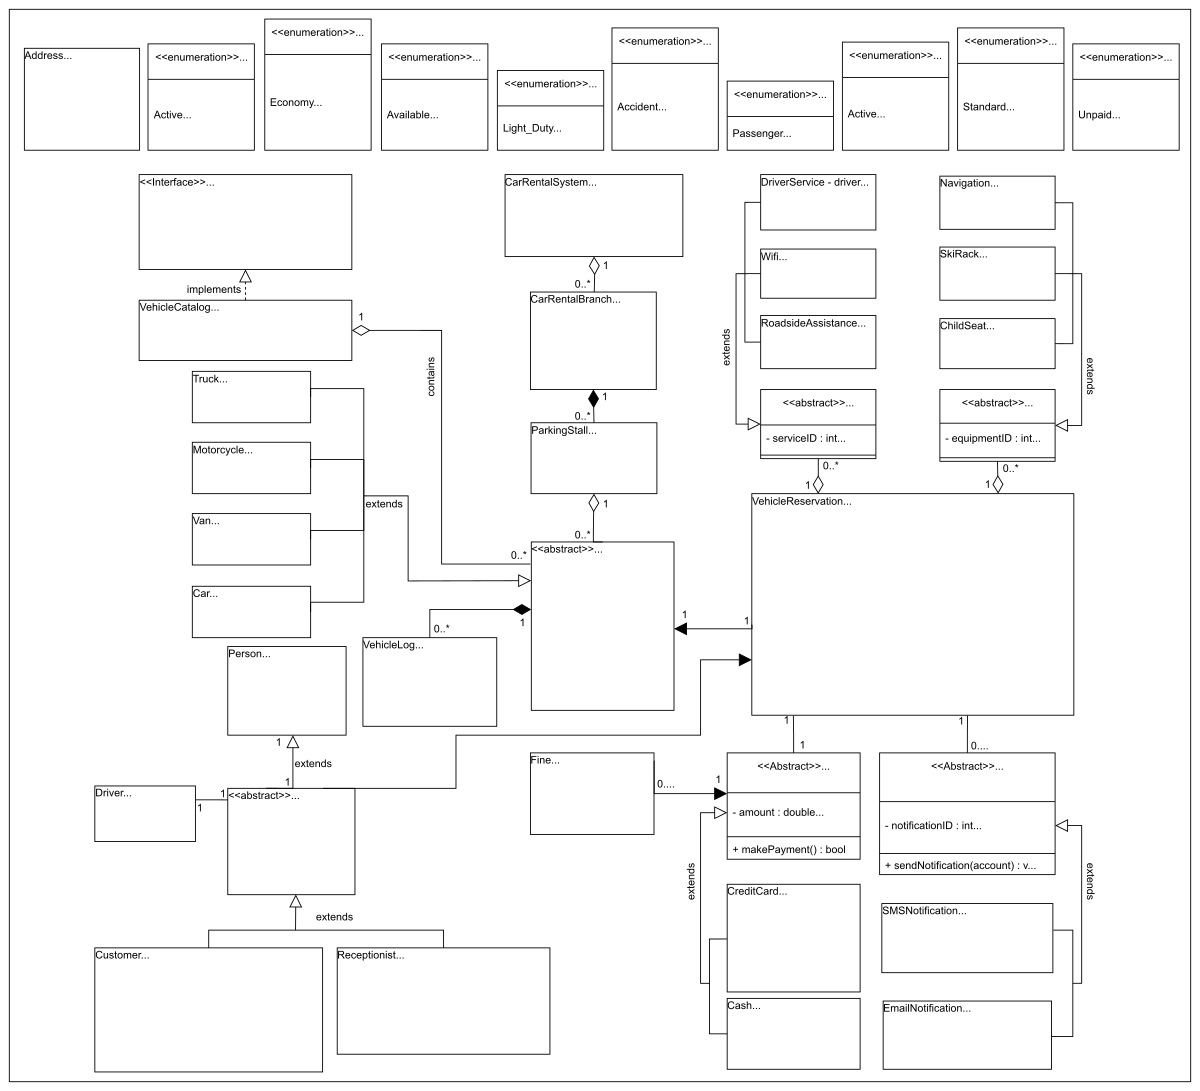
\includegraphics[width=0.5\textwidth]{Images/chapter_15/section_5607380186562560/6663879219085312.png}
 \caption{The class diagram of the car rental system}
\end{figure}

\subsection{Design pattern}\label{MX7PrZF8m5IGmTfFHapJh}
\\
To promote extensibility and adhere to design principles like SRP (Single Responsibility principle) and OCP (Open/Closed principle), we can use the Decorator pattern for dynamic fee calculation and feature extension:

\begin{itemize}
\item
\protect\phantomsection\label{xT9WP6NGjx3YkPnpYuzYX}
\textbf{DiscountDecorator:} Applies discounts to all types of vehicles.
\item
\protect\phantomsection\label{AHUElADefQNyQLhhVbZuB}
\textbf{PeakSeasonDecorator:} Adjusts pricing during peak demand.
\item
\protect\phantomsection\label{7e1_34433NncOmiOtBLa1}
\textbf{DamageFineDecorator:} Calculates fines for returned vehicles with damage.
\item
\protect\phantomsection\label{BjzKia8Qcf1URt2nmem3B}
\textbf{FuelFineDecorator:} Calculates fines for vehicles returned with a partially filled fuel tank.
\end{itemize}
\\
These decorators enable you to add or modify price-related behaviors without changing the underlying vehicle, reservation, or payment classes. Other decorators can be introduced as system needs evolve.
\\
Similarly, we can make several other decorators according to the system's needs. These decorators fulfill the SRP and OCP design principles.

\subsection{AI-powered trainer}\label{8Fmv9eUiBjFgTOcFPh3ww}
\\
At this stage, everything should be clear. If you encounter any confusion or ambiguity, feel free to utilize the interactive AI-enabled widget below to seek clarification. This tool is designed to help you strengthen your understanding of the concepts.

\begin{figure}[htbp]
 \centering
 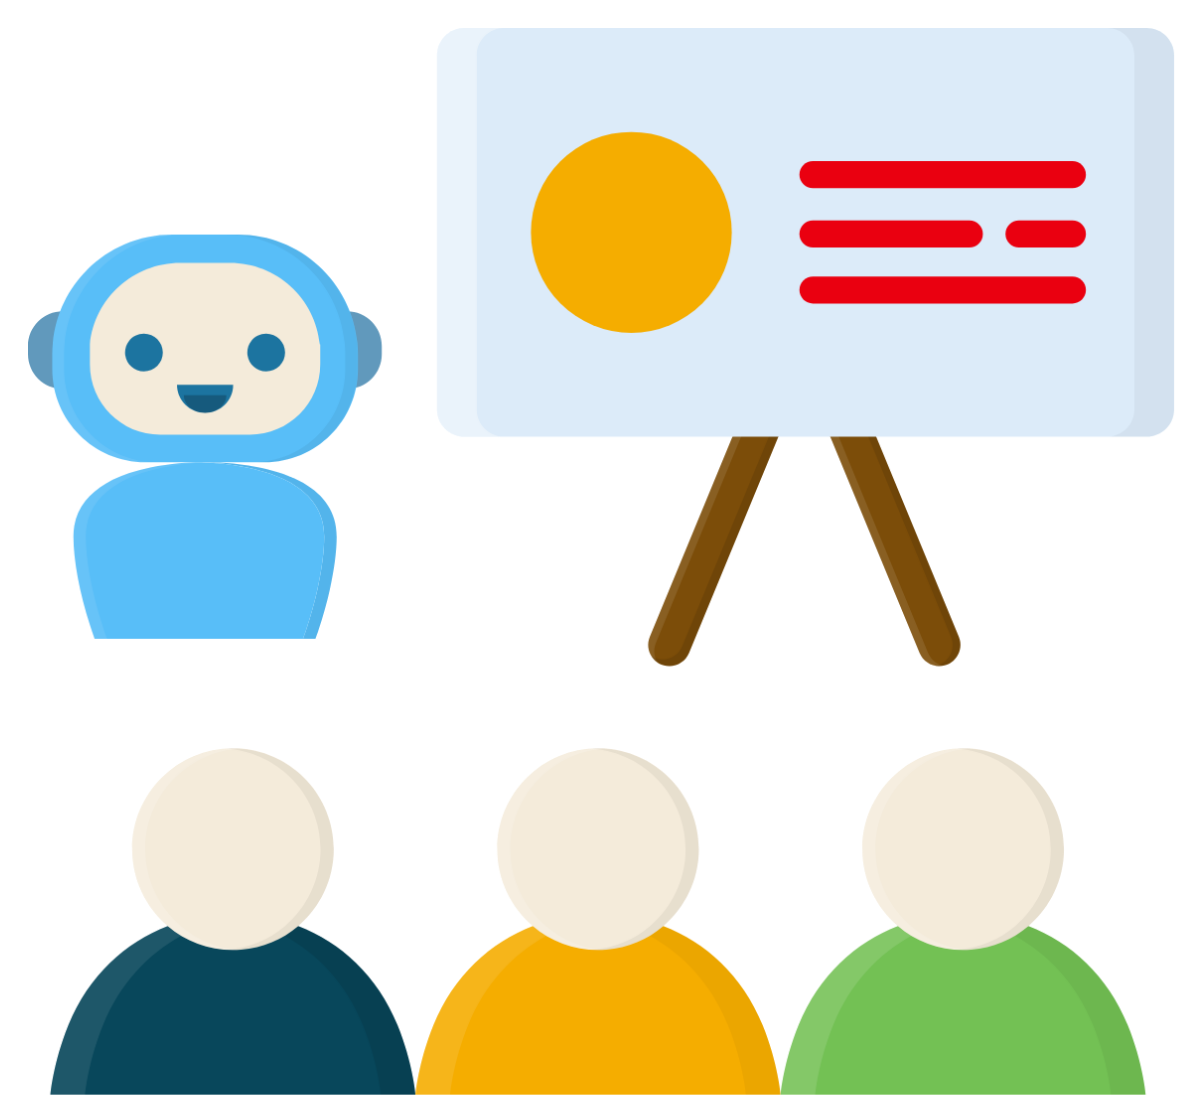
\includegraphics[width=0.15\textwidth]{Images/chapter_15/section_5607380186562560/4813531940519936.png}
 
\end{figure}

\subsection{Additional requirements}\label{szivCGO1_jQ2gCG1SzB9q}
\\
The interviewer can introduce some additional requirements in the car rental system, or they can ask some follow-up questions. Let 's see an example of additional requirements:
\\
\textbf{Barcode scanner:} Each vehicle should have a unique barcode associated with it, and the system should be able to scan the barcode of every vehicle. To fulfill this requirement, we have the class diagram as shown below:

\begin{figure}[htbp]
 \centering
 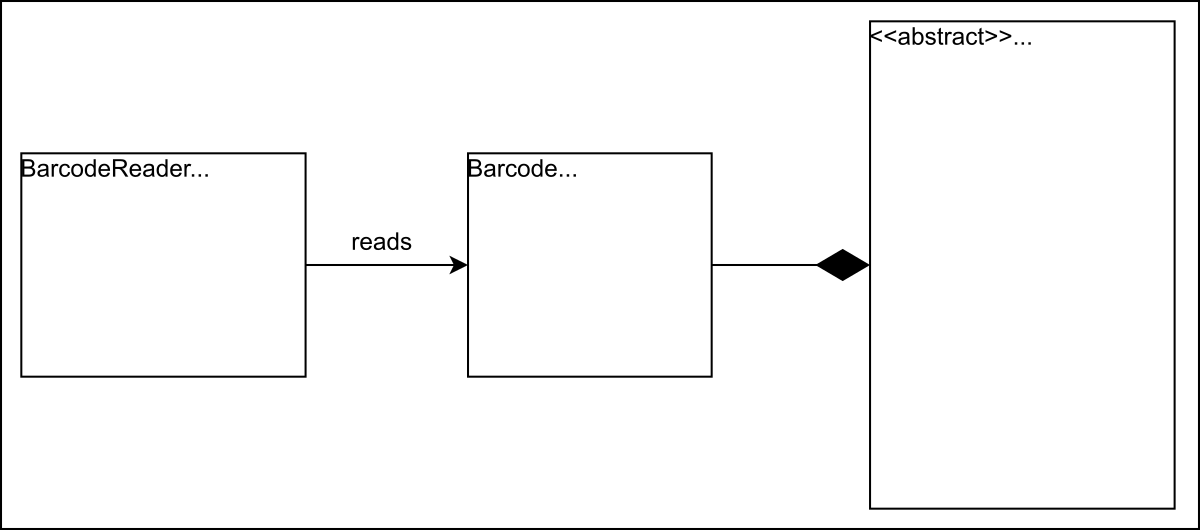
\includegraphics[width=0.5\textwidth]{Images/chapter_15/section_5607380186562560/5270780944580608.png}
 \caption{The class diagram of barcode scanner functionality}
\end{figure}

We have completed the class diagram of the car rental system according to the requirements. In the next lesson, let's design the system's sequence diagram.

% End of section content